\newpage
\section{Theory} \label{theory}
In this section we will outline the basic theory of Principal component analysis, Variational Autoencoders and Generative Adversarial Networks. For the latter two we will do a brief literature review while developing the theory behind the models.

\subsection{PCA}
The first method we will explore is Princinal Component Analysis. PCA is most often thought of at a technique for dimensionality reduction but as we will see here is can also be used for image synthesis.

PCA provide a relatively simple to understand "non-neural" baseline for our exploration of how to use  generative algorithms for face synthesis.

The goal of PCA is to find the Principal Components which are the directions of greatest variance in the dataset. These directions are the eigenvectors or, in this context \emph{eigenfaces}, of the covariance matrix.

Let $\tilde{\mathbf{X}} = \mathbf{X} - \bar{\mathbf{X}}$ then $\mathbf{X}^T\mathbf{X}$ is the covariance matrix we find the eigenfaces the usual way by demanding that $\det(\mathbf{X}^T\mathbf{X} - \lambda) = 0$

Since the matrix of eigenfaces diagonlized the covariance matrix and the fact the covariance of a variable with itself is the variance of that variable we easily see that the eigenvalue of each eigenface is the variance of that eigenface. So once we have found the eigenfaces, we then sort the them after eigenvalue $\lambda$ in order of descending variance.

We can now generate new synthetic faces $F$ by adding a linear combination of the eigenfaces $F_i$ to the mean face $F_m$.
\begin{align}
F  = F_m + \sum_{i} \alpha_i F_i
\end{align}

We explore the results of applying this technique in Section \ref{training} where we will see that the eigenfaces are able to caputure meaningfull informaiton about the data sets.

\subsection{Variational Autoencoders}
% https://www.jeremyjordan.me/variational-autoencoders/
% https://danijar.com/building-variational-auto-encoders-in-tensorflow/
% https://jaan.io/what-is-variational-autoencoder-vae-tutorial/


Variational Autoencoders were first proposed in \textit{Auto-Encoding Variational Bayes} \cite{vae1} and \textit{Stochastic Backpropagation and Approximate Inference in Deep Generative Models} \cite{vae2}

Variational autoencoders build upon normal autoencoders which consist of an encoder $E$ and a decoder $D$. The decoder compresses a datapoint $x$ to s lower dimensional latent representation $z = E(x)$ while the decoder learns the reverse mapping. The network is then then trained to minimize the reconstruction error between an input $x$ and the output $D(E(x))$. 

While the normal autencoder learns a mapping from $x$ to $z$ a variational autoencoder on the other hand learns a probability distribution of the data. 
We assume that the observed variable $\mathbf{x}$ is a sample from the true distribution $p^*(\mathbf{x})$.\cite{vaeintro} 

Our goal is to approximate the true distribution with a model such that
\begin{align}
  p_\theta(\mathbf{x})\approx p^*(\mathbf{x})
\end{align}
Now, in a variational autoencoder the latent variable is drawn from a prior $z\sim p(z)$ wich we choose to be normally distibuted with zero mean and unit standard deviation. We can the then draw datapoint new $x\sim p(x|z)$.The learned joint probability distribution over the data and latens variables is given by
\begin{align}
    p(x,z)=p(x|z)p(z)
\end{align}
Now take $p(x)$ which is refered to at the model \emph{evidence}. It is the integral over the joint distribution
\begin{align}
    p(x)= \int p(xz)dz \int p(x|z) p(z)dz 
    \label{evidence}
\end{align}
Calculting this however is typically intractible since neigther analytic solution or efficient estimators exists. \cite{vaeintro} 

The solution to the intractibility problem is to model the true posterior $p(z|x)$ by a family of distributions $p(z|x)_\theta$ parameterized by the variational parameter $\theta$. We can model $p(z|x)_\theta$ and $p(x|z)_\theta$ by neural networks. The encoder network models $p(z|x)_\theta$ while the decoder network models $p(x|z)_\theta$ We wish to optimize $\theta$ such that $p(z|x)\theta \approx p(z|x)$

From Bayes theorem we get the \emph{posterior}  
\begin{align}
    p(z|x) =\frac{p(x|z)p(z)}{p(x)}
\end{align}

Now to have a metric for how close two probability densities $p$, $q$ are to each other we can use the Kullback-Leibler (KL) divergence which is defined as
\begin{align}
D_{\text{KL}}(p,q) = \int p(x)\log \left(\frac{q(x)}{p(x)}\right) dx =  \mathbb{E}_{x\sim p(x)}\left[ \log\left(\frac{q(x)}{p(x)}\right)\right]
\end{align}

TheKL divergence  is non-negative $D_{\text{KL}}(p,q) \geq 0$ and zero if and only if $p(x) q(x)$. Now the KL divergence  between the modeled posterior $ p_\theta(z|x)$ and the true posterior  $p(z|x)$ is

\begin{align}
    D_{\text{KL}}(p_\theta(z|x),p(z|x)) = \mathbb{E}_{x\sim p(x)} \log\left(\frac{p(x,z)}{p_\theta(z|x)}\right) -  \mathbb{E}_{x\sim p(x)} \left[\log(p(x))\right]
\end{align}

Now the model evidence from eq. \ref{evidence} is intratable so we cannot compute it directly. The first term is called the "Evidence Lower BOund" 

\begin{align}
    \text{ELBO}(x) = \mathbb{E}_{x\sim p(x)} \log\left(\frac{p(x,z)}{p_\theta(z|x)}\right)
\end{align}
Since we now can rewtire the model evicende as 
\begin{align}
    \log(p(x)) = \text{ELBO}(x) +  D_{\text{KL}}(p_\theta(z|x),p(z|x))
\end{align}
And since the KL divergence is non-negative this means that that minimizing the Kullback-Leibler divergence is equivalent to maximizing the ELBO. Thus we can make the ELBO our loss function $-l_\theta(x)=\text{ELBO}(x)$. 

This achieves two things we care about\cite{vaeintro}: 

\begin{enumerate}
    \item It will maximize the marginal likelihood $p_\theta(x)$.
This means that our generative model will become better.
    \item It will minimize the KL divergence between $q_\theta(z|x)$ and $q_\theta(z|x)$ so the model posterior become closer to the true posterior.
\end{enumerate}


% The Kullback-Leibler divergence is defined as by
% \begin{align}
% D_{\text{KL}}(p_\theta,q_\phi) = -\sum_{\mathbf{x}\in\mathcal{X}}p_\theta(\mathbf{x})\log \frac{q_\phi(\mathbf{x})}{p_\theta(\mathbf{x})}
% \end{align}


% Now, how do we go about actually modeling this distribution $p_\theta(\mathbf{x})$?. We can use Neural networks to parametrize the distribution.


% \textit{Generating Diverse High-Fidelity Images with VQ-VAE-2}\cite{vqvae2}





\subsection{Generative Adversarial Networks.}

Generative Adversarial Networks (GANs) have been shown to be able to create be able to generate photo realistic images of human faces.\cite{progan}

There has been proposed several improvements and variations of the original GAN architecture proposed in 2014 by Ian Goodfellow et al.\cite{gan}.

The premise of GANs is to play minmax game between two competing neural networks. We simultaneously train a discriminator $D$ and a generator $G$.
The discriminator $D$ is a binary classifier whose objective is classify whether a show example image is coming from the data distribution $p_D$ or from the generated $p_G$ distribution. In the original paper discriminator and generator architectures were both multilayer perceptrons.

The original value function, is given by
\begin{align}
\min_G \max_D \mathbb{E}_{\mathbf{x}\sim p_{\text{data}}(\mathbf{x})}
\left[\log D(\mathbf(x))]\right]+
\mathbb{E}_{\mathbf{z}\sim p_{\mathbf{z}}(\mathbf{z})}
\left[\log (1-D(G(\mathbf(z)))]\right]
\end{align}
Here the $G$ tries to minimize $\mathcal{L}$ while the $D$ tries to maximize it.

Since $D$ is taking a data point (image) $\mathbf{x}\in X$ and giving the probability that image is real or generated, it is a mapping $D:X \to (0,1)$. We define the generator as to depend on a latent variable $\mathcal{z}\in Z$ such that $G(\mathcal{z})$ is a mapping $G:Z\to X$.

In \textit"{Unsupervised Representation Learning with Deep Convolutional Generative Adversarial Networks"}(2015) (DCGAN)\cite{dcgan} the authors outlines a set of guidelines to improve the training stability of GANs among them are using convolutional layers, using the RELU activation in all layers i the generator except in the output layer which uses $\tanh$. In the discriminator the activation function is  the LeakyRELU activation which is defined as

\begin{align}
  \text{LeakyRELU}(x) =
  \begin{cases}
    x & \text{if}\quad x\geq0\\
    0.1x & \text{if}\quad x<0
  \end{cases}
\end{align}

where the "normal" RELU just outputs $0$ for $x<0$. The paper also proposes to do batch normalization in both the generator and the discriminator and to replace any pooling layers with strided convolutions. Batch normalization means that we normalize every input feature of a layer to have zero mean and unit variance.\footnote{\url{https://sthalles.github.io/advanced_gans/}}. A stride in a convolutional layer defines the distance between the spatial locations where the convolution kernel is applied.

In the paper \textit{"Progressive Growing of GANs for Improved Quality, Stability, and Variation"}(ProGan)\cite{progan} the authors used GANs to generate photorealistic images from CelebA-HQ a high quality version of the original CelebA dataset.\cite{celebA}. This work also uses convolutional layers and the main improvement is to progressively grow the generated images starting from a low resolution and then gradually add more layers to the generator and discriminator networks to produce higher resolution images.

In \textit{"Large Scale GAN Training for High Fidelity Natural Image Synthesis"}(BigGAN) \cite{biggan} the authors find progressive growing is unnecessary even for the largest images they considered which was 512 by 512 color images. They trained their GAN on imagenet which consists of over 14 million images which are annotated in the in a tree structure.\cite{imagenet} This is by far the GAN which has been trained on the largest dataset that I could find during the review of recent GAN literature.
% In SA-GAN\cite{sagan}

In \textit{A Style-Based Generator Architecture for Generative Adversarial Networks}(2018)\cite{stylegan} the authors improved the ProGan model by including elements from the style transfer literature. Particularly instead of feeding the latent vector $z\in\mathcal{Z}$ directly into the generator via a fully connected layers, StyleGAN introduces a non-linear mapping network $f:\mathcal{Z}\to\mathcal{W}$ which encoded the input latent vector $z$ into an intermediate vector $w$.

The vector $w$ then controls the generator through adaptive instance normalization (AdaIN) at each convolution layer.
AdaIN, first proposed in 2017 \cite{adain} is given by

\begin{align}
  \text{AdaIN}(\mathbf{x},\mathbf{y}) = \mathbf{y}_s \frac{\mathbf{x}-\mu(\mathbf{x})}{\sigma{\mathbf{x}}}+\mathbf{y}_b
\end{align}

AdaIn uses a "learned affine transformation” $A$ that maps the latent  vector $\mathbf{y}$ onto two scalars $A(\mathbf{w})= \mathbf{y}=(\mathbf{y}_s,\mathbf{y}_b)$ here $s$ stands for scale, and $b$ stands for bias.

\begin{wrapfigure}{r}{5.5cm}
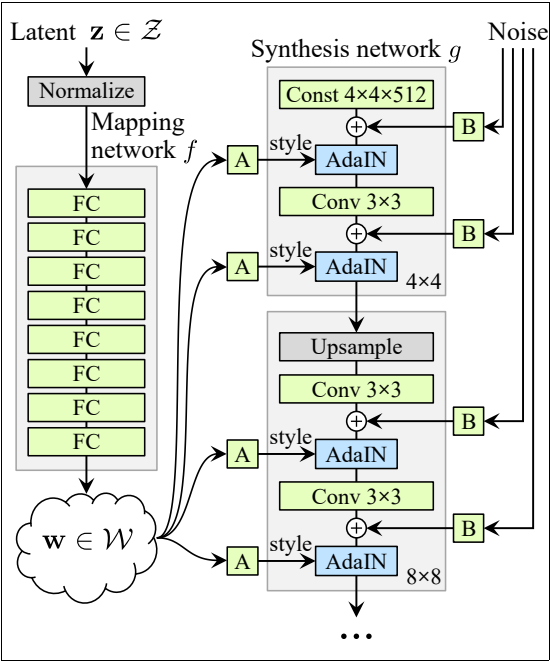
\includegraphics[width=5.5cm]{fig/stylegan-arch}
\caption{Summary of the StyleGAN Generator Model Architecture.
Taken from: A Style-Based Generator Architecture for Generative Adversarial Networks.\cite{stylegan}}
\label{stylegan-arch}
\end{wrapfigure}


In the StyleGAN paper the authors also introduce a new data set called FlickrFaces-HQ (FFHQ) \footnote{Made public here: \url{https://github.com/NVlabs/ffhq-dataset}}, which consists of 70,000 images with even more variation than the CelebA-HQ dataset.\cite{stylegan} We will use a lower resolution subset of this data set to train our own models in the next section.  

In the paper \textit{Interpreting the Latent Space of GANs for Semantic Face Editing}(2019)\cite{interfacegan} is was shown that the latent space of StyleGAN is disentangled to a high degree and it is possible to find subspaces in the latent space that encode different semantic features.

Since it has been shown that for a "well-trained" GAN one can linearly interpolate beween to latent vectors  $z_1$ and $z_2$ and the resultant generated images $G(z_1)$ and $G(z_2)$ would also vary smoothly. We can for example smoothly morph an image of a man intro the face of a woman by interpolating bewteen the two latent vectors.   

In the paper the central assumption that is true for any binary semantic attribute (e.g., male  and female or smile and no smile).\cite{interfacegan} Therefore there will exist a hyperplane in the latent space serving as the separation boundary.
These  separation boundary were  found by first generating a set of random images by sampling the latent vector from the normal distribution and linear SVM on the semantic attribute we are interested in.
In the paper they trained 5 indepentent SVMs on pose,smile,age,gender and eyeglasses using 40K random samples.

Having found the separating hyperplane in the latent space the normal vector of this hyperplane gives us a semantic direction in the latent space. which we can use to to semandic face diting which we will do in section \ref{stylegan}









% In SA-GAN\cite{sagan}
%
% \section{Inception Score}
% \url{https://machinelearningmastery.com/how-to-implement-the-inception-score-from-scratch-for-evaluating-generated-images/}
%

% \section{Principal Component Analasyis. }

% \paragraph{Face Aging}
% \textit{Face Aging With Conditional Generative Adversarial Networks} (2017) \cite{faceaging}

% \section{3D Reconstruction}
%
% \textit{Projective Structure from Facial Motion}(2017)\cite{ProjectiveStructure}
%
% \textit{Apathy is the Root of all Expressions}(2017)\cite{apathy}
%
% In the paper \textit{"Large Pose 3D Face Reconstruction from a Single Image via Direct Volumetric CNN Regression"}(2017)\cite{largepose}
% the authors used a Convolutional Neural Network to reconstruct the 3D facial geometry from just a single image. The model work under arbitrary poses
% and expressions and without the need of a 3D Morphable Model.
